\section{Evolving Neural Networks for a Flatland Agent}
\subsection{EA-parameters}
\begin{center}

\begin{tabular}{p{5cm} | r}
Parameter & Value \\
\hline
Population & 75 \\
Maximum iterations & 200 \\
Elitism & 5 \\
Tournament size & 10 \\
Tournament epsilon & 0.2 \\
Mutation percent & 0.05 \\
Crossover rate & 0.2 \\
\hline
\end{tabular}
\end{center}

\subsection{Fitness function}
$f(x) = positive - negative$

\subsection{ANN design}
\begin{figure}[h!]
  \centering
    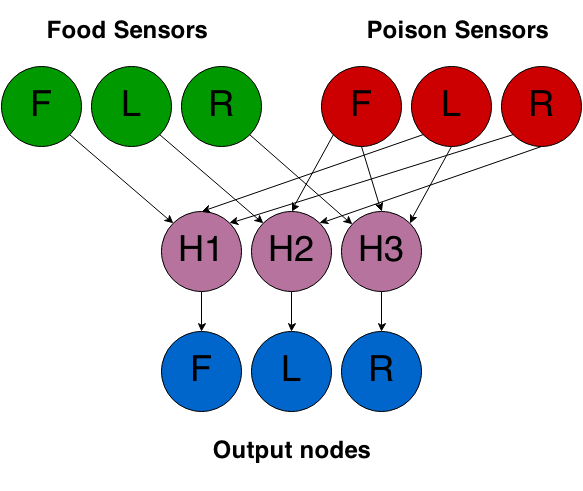
\includegraphics[width=0.5\textwidth]{img/Flatland_network}
\end{figure}

Three hidden nodes represents the layer between the input sensors and the output nodes. The main idea of the hidden nodes is to understand that the poison is negative and food is positive for the final outputs. The food input sensors is linked to the "same" hidden node, while the poison input sensors is linked to the "opposite" hidden node. 

The weights in this artificial neural network can have values $[-1, 1]$ 

\subsection{Static vs dynamic runs}
Hard coded runs vs $FPD(x, y)$ runs

